%
%      File Name : HW1.tex
%  Creation Date : 12-08-2013
%  Last Modified : Fri Aug 23 17:08:07 2013
%

\documentclass[pdftex,11pt]{article}
\usepackage{url}
\usepackage{graphicx}
\usepackage{hyperref}
\usepackage{latexsym,amssymb}
\usepackage{amssymb,amsmath}

\usepackage[english]{babel}
\usepackage{array}
\usepackage{multirow} 
\usepackage{fontspec}
%  \setmainfont{Arial}
%  \setmainfont[Ligatures=TeX]{Arial}

\newcommand{\sourcefile}{\path}
\hypersetup{colorlinks=false}

\hypersetup{
pdftitle={MATH 4650 :: 001 and 003 :: Numerical Analysis},
pdfauthor={Julien Langou}, 
} 

\setlength{\oddsidemargin}{-0.5in}
\setlength{\evensidemargin}{-0.5in}

\setlength{\textwidth}{7.4in}
\setlength{\textheight}{10.0in}

\setlength{\topmargin}{-0.75in}
\setlength{\headheight}{0pt}
\setlength{\headsep}{0pt}

\setlength{\parindent}{0pt}

\begin{document}

\thispagestyle{empty}
\pagestyle{empty}

\textbf{MATH 4650} 

\vspace{2cm}

\textbf{\color{blue} Sauer.0.5.6}\\

{\color{blue} Note: In this exercise, we pretty much do not consider round-off
errors.  For example, we will assume that the values returned by matlab when
evaluating $f(x)=x^{-2}$ are exact.  This is justified because our
approximation errors (using Taylor polynomials) are much larger than the
round-off errors. We will see some limitations (when round-off errors are not
negligible any longer) at the end of the exercise.  } 

\renewcommand{\theenumi}{\alph{enumi}}
\begin{enumerate}\addtolength{\itemsep}{1.00\baselineskip}

\color{red}\item
Find the Taylor polynomial of degree 4 for $f(x)=x^{-2}$ about the point $x_0=1$.\\
\color{black}

We recall the formula for the Taylor polynomial of degree 4 of a function $f$ at $x_0$:
$$p_4(x) = 
f(x_0) 
+ f'(x_0) (x-x_0)
+ \frac{1}{2!} f''(x_0) (x-x_0)^2
+ \frac{1}{3!} f^{(3)}(x_0) (x-x_0)^3
+ \frac{1}{4!} f^{(4)}(x_0) (x-x_0)^4.
$$

We want to use this formula for $f(x)=x^{-2}$ and $x_0=1$.
First, we compute the first four derivatives of $f(x)=x^{-2}$:
$$
f(x) = \frac{1}{x^2},\quad 
f'(x) = -\frac{2}{x^3},\quad 
f''(x) = \frac{3!}{x^4},\quad 
f^{(3)}(x) = -\frac{4!}{x^5},\quad 
f^{(4)}(x) = \frac{5!}{x^6}.
$$

Then, we evaluate these derivatives at $x_0=1$:
$$
f(1) = 1,\quad 
f'(1) = -2,\quad 
f''(1) = 3!,\quad 
f^{(3)}(1) = -4!,\quad 
f^{(4)}(1) = 5!.
$$

Finally, we substitute $f(1)$, $f'(1)$, $f''(1)$, $f^{(3)}(1)$, and
$f^{(4)}(1)$ in the formula for $p_4(x)$ and obtain:
$$
p_4(x) = 
1 - 2 (x-1) + 3 (x-1)^2 - 4 (x-1)^3 + 5 (x-1)^4.
$$

\color{red}\item
Use the result of (a) to approximate $f(0.9)$ and $f(1.1)$.\\
\color{black}

In MATLAB, using $p_4(x)= 1 - 2 (x-1) + 3 (x-1)^2 - 4 (x-1)^3 + 5 (x-1)^4$, 
we obtain:
$$p_4(0.9) = 1.2345 \quad \textmd{and} \quad p_4(1.1) = 0.8265.$$

In MATLAB, using the definition $f(x)=x^{-2}$, we can also compute
$$f(0.9) \approx 1.23456790123457 \quad \textmd{and} \quad f(1.1) \approx 0.826446280991735.$$

We see that $p_4(0.9)$ is a ``reasonable'' approximation of $f(0.9)$, and
$p_4(1.1)$ is a ``reasonable'' approximation of $f(1.1)$.

\color{red}\item
Use the Taylor remainder to find an error formula for the Taylor polynomial.
Give error bounds for each of the two approximations made in part (b). Which of
the two approximations in part (b) do you expect to be closer to the correct
value?\\
\color{black}

We have $x_0=1$. If $x$ is any real number in $(0,\infty)$, then the function 
$f(x)=x^{-2}$ is $k+1$ times continuously differentiable in either the interval 
$[x,x_0]$ or $[x_0,x]$, whichever makes sense. The assumptions of the
Taylor's Theorem with Remainder (Theorem 0.8 page 21) are therefore satisfied.

Taylor's Theorem with Remainder tells us that there exists $c$ in between $x$ and $x_0$ such that
$$f(x) = 
f(x_0) 
+ f'(x_0) (x-x_0)
+ \frac{1}{2!} f''(x_0) (x-x_0)^2
+ \frac{1}{3!} f^{(3)}(x_0) (x-x_0)^3
+ \frac{1}{4!} f^{(4)}(x_0) (x-x_0)^4
+ \frac{1}{5!} f^{(5)}(c) (x-x_0)^5.
$$
We note that $c$ depends on $x$. Sometimes we write $c_x$ which is actually a good thing.
We repeat: for each different $x$ in the formula above, we have a different $c$.

In other words, using $x_0=1$, $p_4(x)= 1 - 2 (x-1) + 3 (x-1)^2 - 4 (x-1)^3 + 5 (x-1)^4$, 
and the fact that $f^{(4)}(x) = - (6!)x^{-7}$, we obtain that
there exists $c$ in between $x$ and 1 such that:
$$ f(x) = p_4(x) - \frac{6}{c^7} (x-1)^5.$$

This enables to control the error made by approximating $f(x)$ with $p_4(x)$ with the formula:
$$ | f(x) -  p_4(x) | \leq  \frac{6}{c^7} |x-1|^5,
\quad \textmd{where }c\textmd{ is in between }x\textmd{ and 1}.$$

Assume that $x>1$, (so we use the formula $p_4(x)$ to approximate $f(x)$ when $x$ is on the right of 1,) then
since $c$ is in the interval $(1,x)$, 
we have $1<c<x$  and so $x^{-7}<c^{-7}<1$, the left part is of interest:
$$\frac{1}{c^7} < 1 $$
and so we obtain a new error bound (without $c$) as:
$$ | f(x) -  p_4(x) | \leq  6 (x-1)^5.$$

Assume that $0<x<1$, (so we use the formula $p_4(x)$ to approximate $f(x)$ when $x$ is on the left of 1,) then
since $c$ is in the interval $(x,1)$, 
we have $x<c<1$  and so $1<c^{-7}<x^{-7}$,  the left part is of interest:
$$\frac{1}{c^7} < \frac{1}{x^7} $$
and so we obtain a new error bound (without $c$) as:
$$ | f(x) -  p_4(x) | \leq  6 \frac{(1-x)^5}{x^7}.$$

We conclude by looking at the relative error bound:
$$  \textmd{rel\_err}(x) = \frac{| f(x) -  p_4(x) |}{|f(x)|} \leq  \textmd{upp\_rel\_err}(x) = \left\{ \begin{array}{l}  6 x^{-5}(1-x)^5, \textmd{ if }0<x\leq 1\\  6x^{2} (x-1)^5, \textmd{ if }1\leq x \end{array}\right..$$

For $x=0.9$, the bound tells us that
$$ \textmd{rel\_err}(0.9) = | f(0.9) -  p_4(0.9) |/|f(0.9)  \leq \textmd{upp\_rel\_err}(0.9) = 1.0e-04.$$

For $x=1.1$, the bound tells us that
$$ \textmd{rel\_err}(1.1) = | f(1.1) -  p_4(1.1) |/|f(1.1)  \leq \textmd{upp\_rel\_err}(1.1) =  7.3e-05.$$

We expect $p_4(1.1)$ to be relatively closer to $f(1.1)$ than $p_4(0.9)$ is to $f(0.9)$

(IMPORTANT: Note that our expectation might very well not happen. We know that
our upper bound for the relative error at 1.1 is smaller than our upper bound
for the relative error at 0.9. We cannot conclude that the relative error at
1.1 is smaller than the relative error at 0.9.)

\color{red}\item
Use a calculator to compare the actual error in each case with your error bound
from part (c).\\
\color{black}

$$ \textmd{rel\_err}(0.9) = | f(0.9) -  p_4(0.9) |/|f(0.9)  \approx 6.5e-5.$$
$$ \textmd{rel\_err}(1.1) = | f(1.1) -  p_4(1.1) |/|f(1.1)  \approx 7.5e-5.$$

We obtain the reverse that what we were expecting. (This is fine.)

\end{enumerate}

\textbf{Figure below:} The red curve is the function $f(x)=x^{-2}$ which we try to
approximate. Blue points represent the function $p_4$ (Taylor polynomial of $f$
at $x_0=1$).  We see that $p_4$ is a ``good'' approximation of $f$ around the
point $x_0=1$.

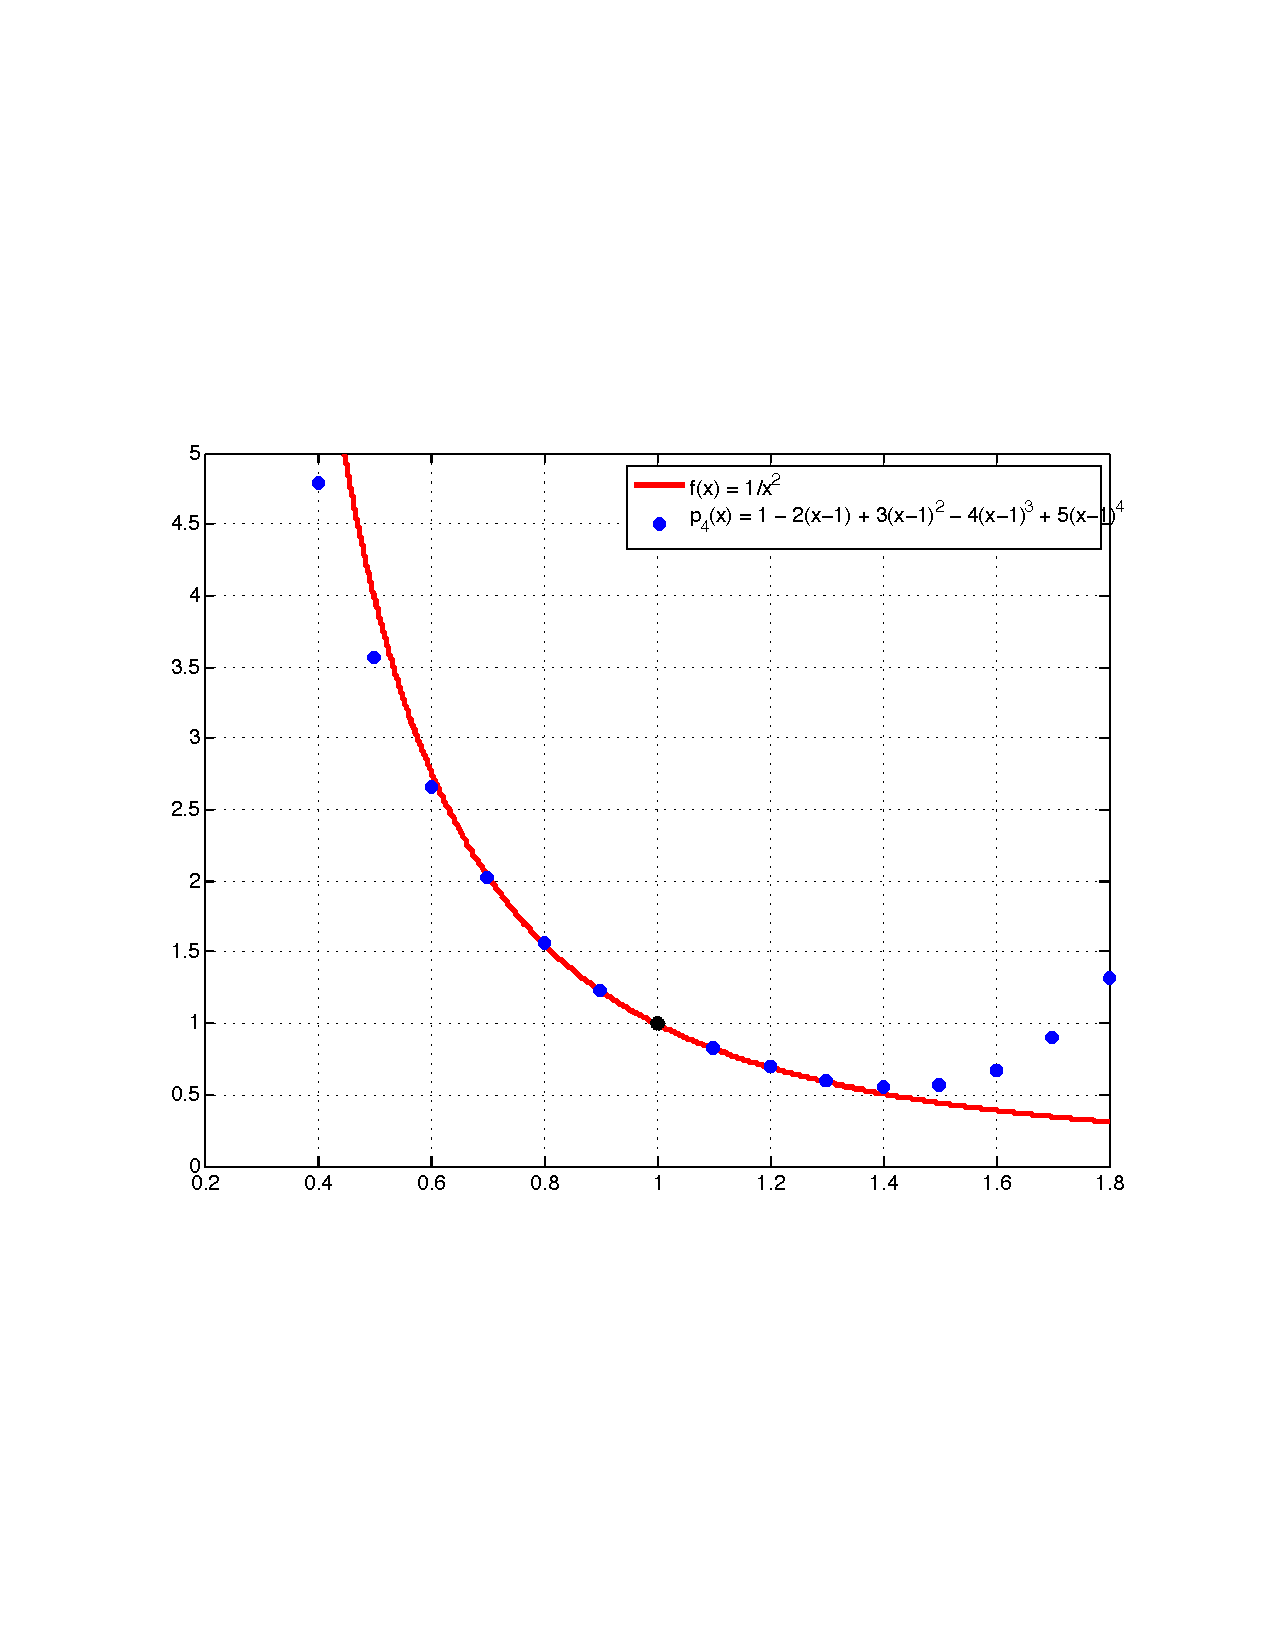
\includegraphics[width=.7\textwidth]{EX_0_5_6_fig1}

\textbf{Figure below:} This represents the relative error
($\textmd{rel\_err}(x)$) (blue dots) and our upper bound on the relative error
($\textmd{upp\_rel\_err}(x)$) (red curve). (1) We see that the relative error
is always below its upper bound. It is a good thing! Of course, the upper bound
is above whatever it is bounding! (2) We see that the relative error and its
upper bound are close. This is not obvious, but this is a good thing, this
means that our upper bound is sharp.  (3) We see that the relative error and
the error bound goes to zero when x goes to $x_0=1$. This is expected.  (3)
Please understand that in general we do not know the relative error.  (So we do
not know the blue dots.) We only know the error bound. To be able to compute
the relative error, we need to know the true quantity. But, if we know the true
quantity: why would we ever compute an approximation to it?  Why do we do it
here? Well, because this is a good numerical analysis exercise! And we will see
why this very useful later in the semester.

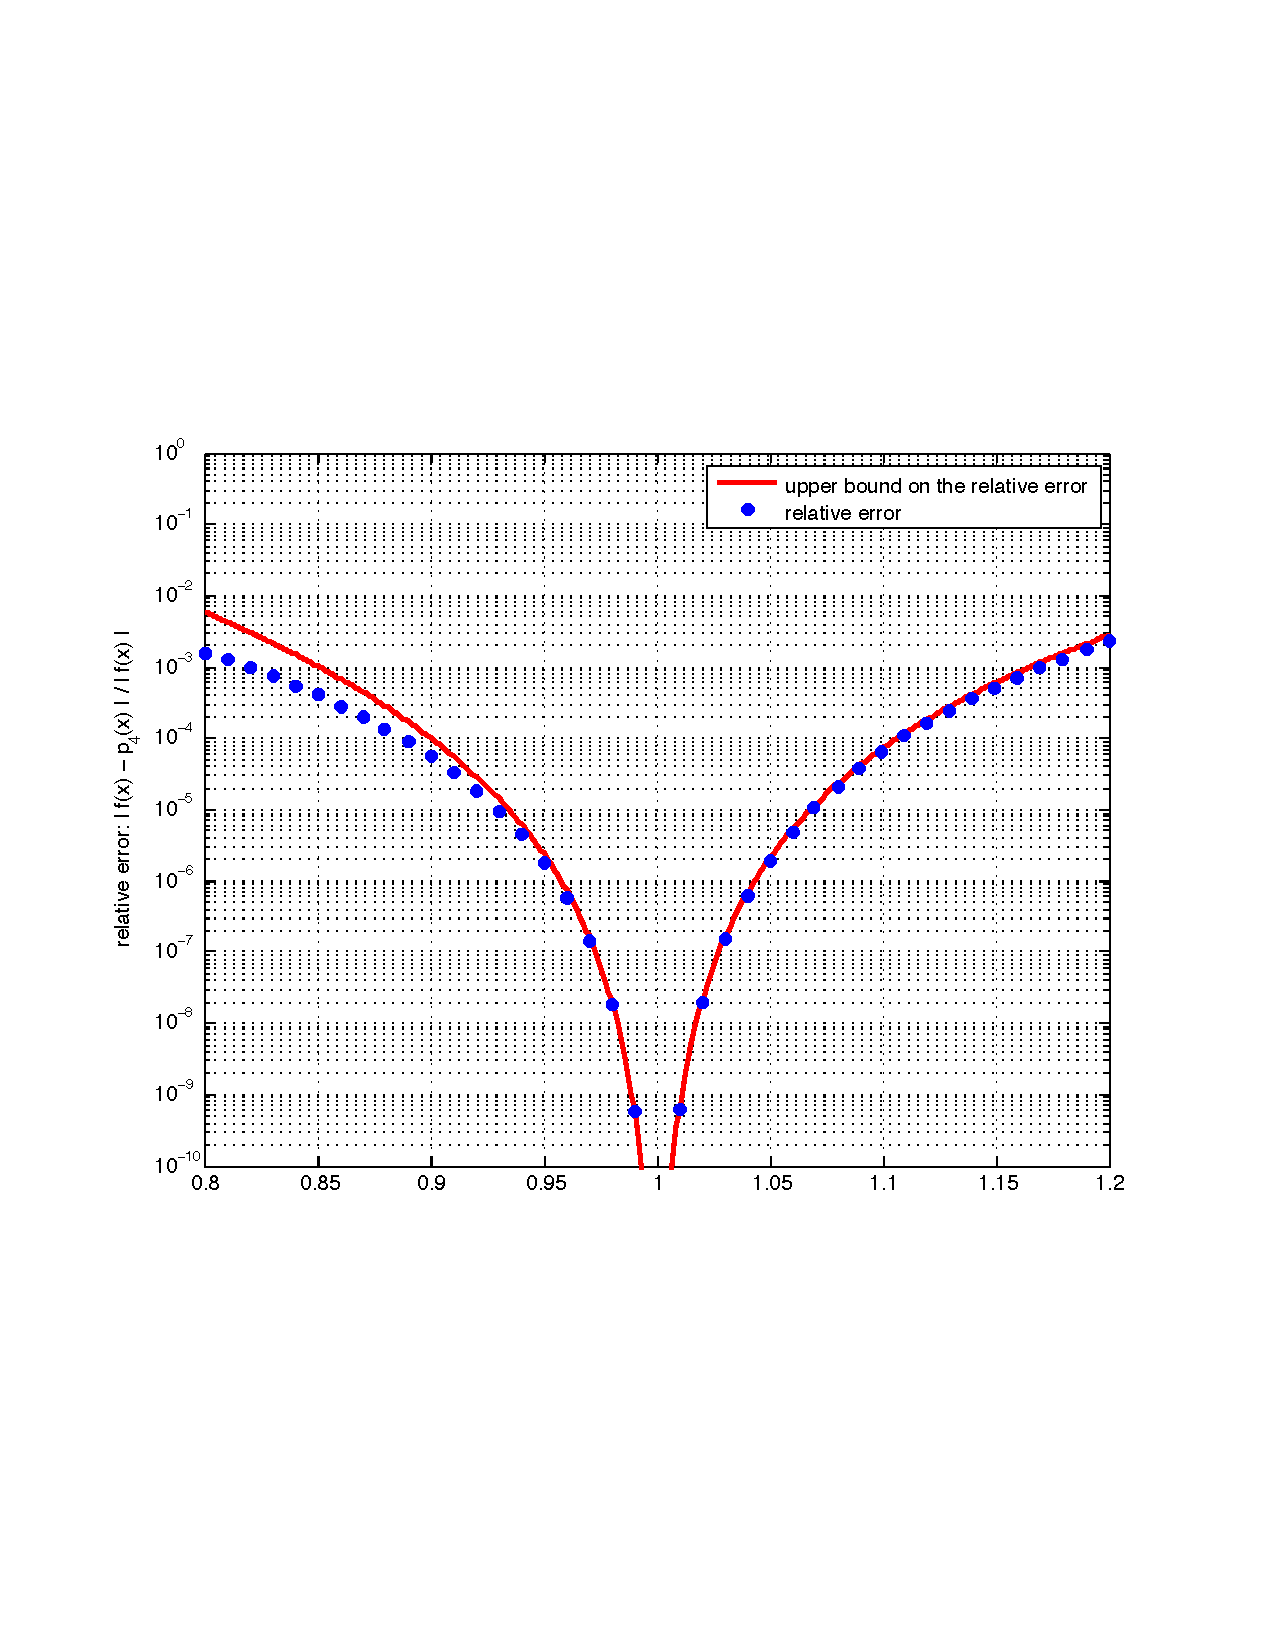
\includegraphics[width=.7\textwidth]{EX_0_5_6_fig2}

\textbf{Figure below:} We only look on the right of $x_0=1$. We look at the
error for points of the form $x=1+h$.  The x-axis is $h$, the y-axis is the
error bound. Note: at some point we see that we have round-off error kicking
in.  Our upper bound (red line) is below our computed errors! This makes no
sense. This is because our computed errors are limited by the machine accuracy
(about $10^{-16}$).

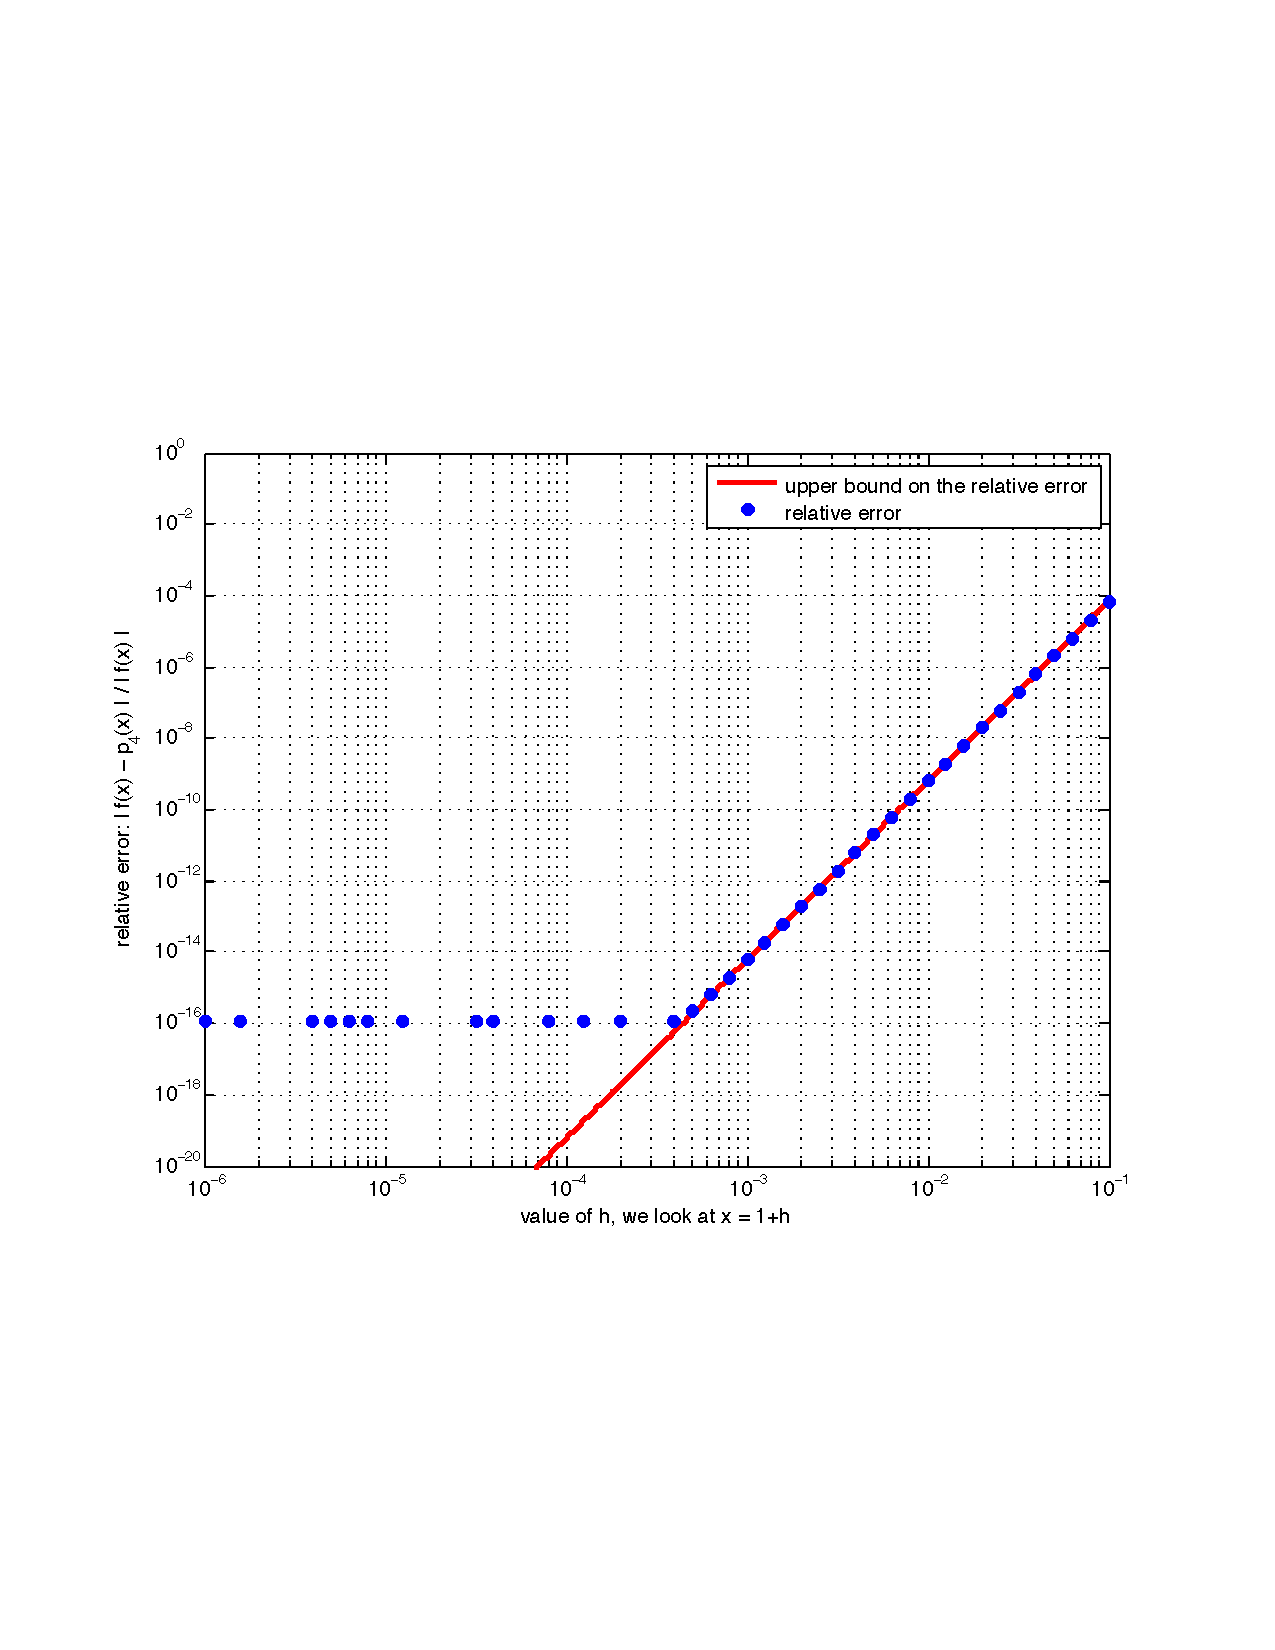
\includegraphics[width=.7\textwidth]{EX_0_5_6_fig3}


\textbf{\color{blue} Beyond the exercise.} 

We can also study and compare various orders of approximation.

We can approximate the function $f(x)=x^{-2}$ around $x_0=1$ by simply the constant function:
$$p_0(x) = 1.$$ 
This is kind of crude. Nevertheless, the closer $x$ gets to $1$ the better, and, at $1$, the approximate quantity is actually exact. 
This is a 0th-order approximation. The accuracy of the formula is $\mathcal{O}(h)$ where $h=|x-1|$.

A better approximation of the function $f(x)$ around $x_0=1$ is the linear function:
$$p_1(x) =  1 - 2 (x-1).$$
This is better. 
This is a 1st-order approximation. The accuracy of the formula is $\mathcal{O}(h^2)$  where $h=|x-1|$.

Etc. The more term the better the approximation. $p_4(x)$ is a fourth order approximation of $f$ at $x_0=1$  and the accuracy of the formula is $\mathcal{O}(h^5)$  where $h=|x-1|$.\\

\textbf{Figure below:} The black line is the function $f(x)=x^{-2}$ and we have plotted 0-th order, 1st order, 2nd order, etc. approximations at  $x_0=1$.

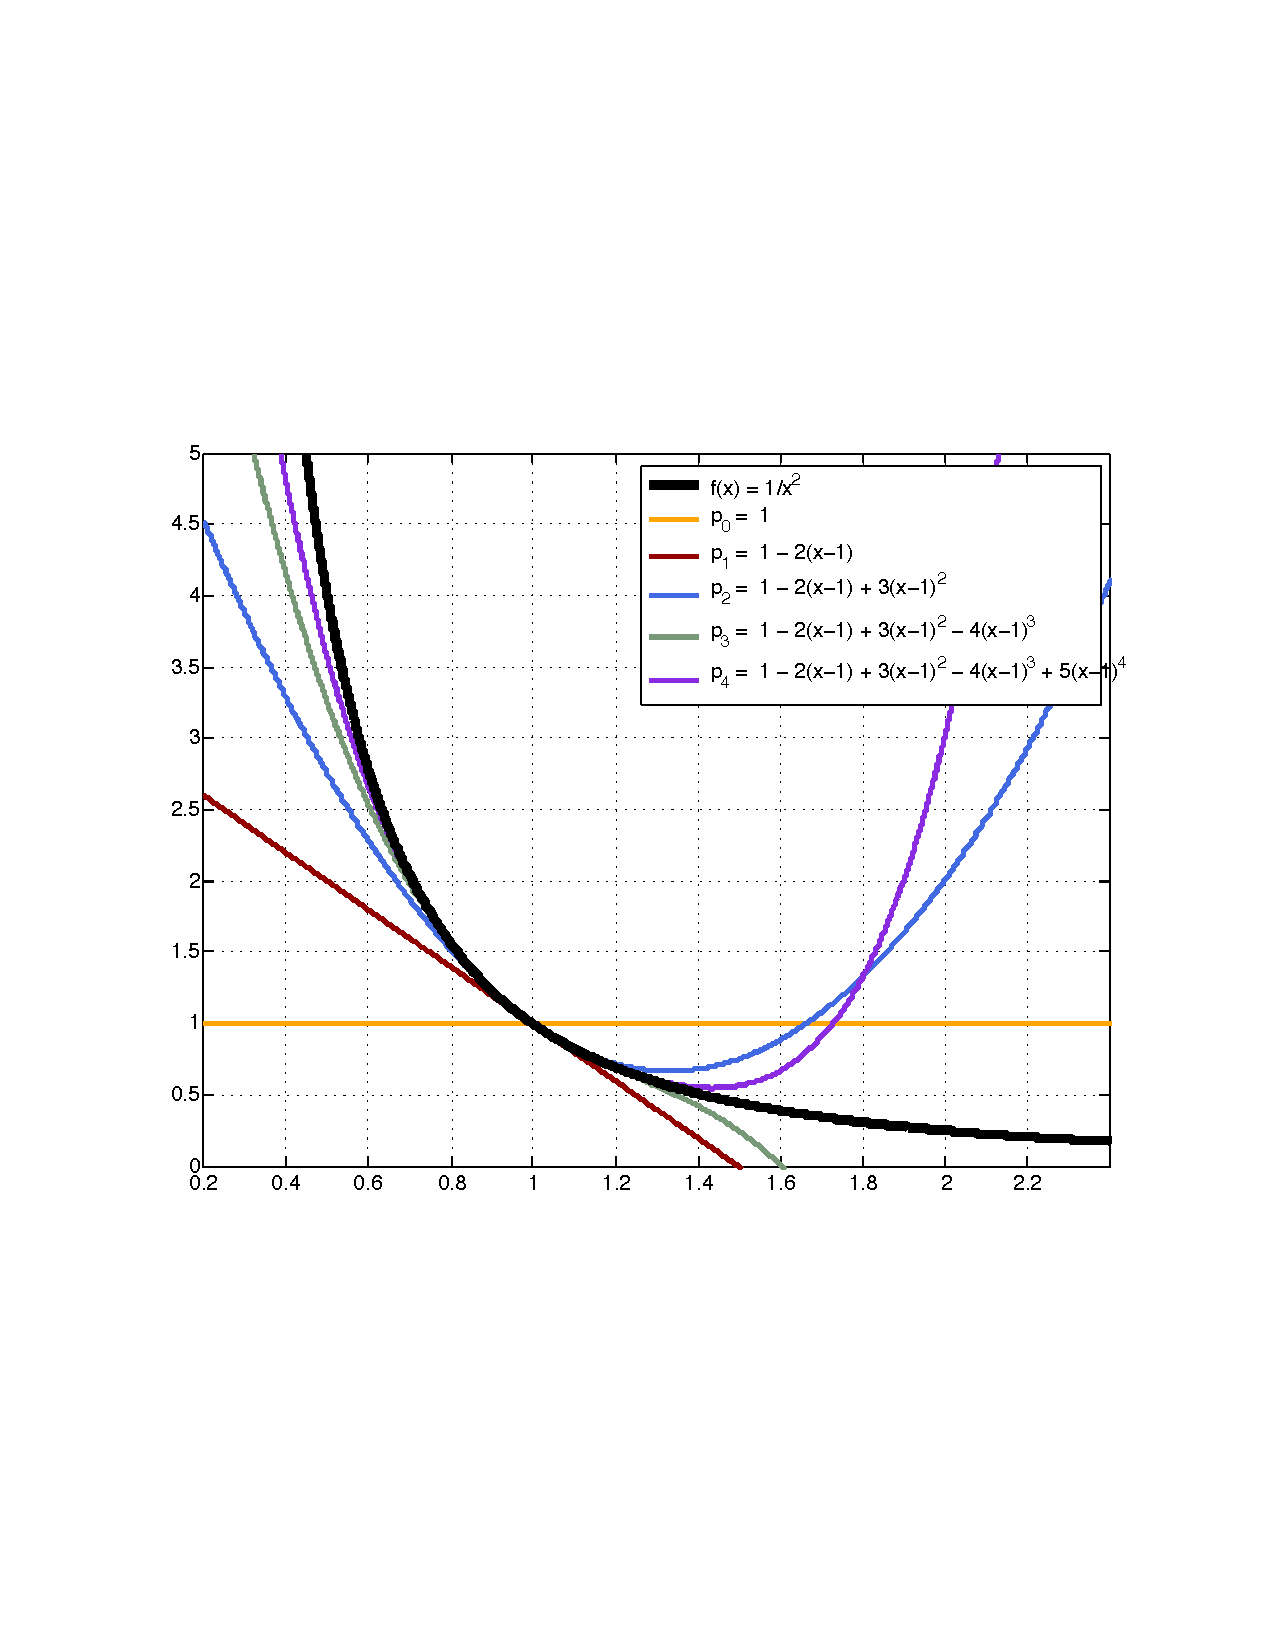
\includegraphics[width=.7\textwidth]{EX_0_5_6_fig4}


\textbf{Figure below:} This is an important curve. This is error as a function
of $h$ for different schemes. The yellow line means $O(h)$-scheme, means 0th
order. The red line means $O(h^2)$-scheme, means 1st order, etc. Let us look at
$h=10^{-3}$ for example. When $h=10^{-3}$, we see that the 0th order scheme ($p_0$,
yellow line) has an error of $10^{-3}$ -- more or less -- which corresponds to
$\mathcal{O}(h)$.  when $h=10^{-3}$, we see that the first order scheme ($p_1$,
red line) has an error of $10^{-6}$ -- more or less -- which corresponds to
$\mathcal{O}(h^2)$.  When $h=10^{-3}$, we see that the second order scheme ($p_2$,
blue line) has an error of $10^{-9}$ -- more or less -- which corresponds to
$\mathcal{O}(h^3)$.  When $h=10^{-3}$, we see that the third order scheme ($p_3$,
green line) has an error of $10^{-12}$ -- more or less -- which corresponds to
$\mathcal{O}(h^4)$.  When $h=10^{-3}$, we see that the third order scheme ($p_4$,
purple line) has an error of $10^{-15}$ -- more or less -- which corresponds to
$\mathcal{O}(h^5)$.  If we change $h$ and look at $h=10^{-4}$ (for example), then
we see $10^{-4}$, $10^{-8}$, $10^{-12}$, and then limited by $10^{-16}$ which is the
machine precision.

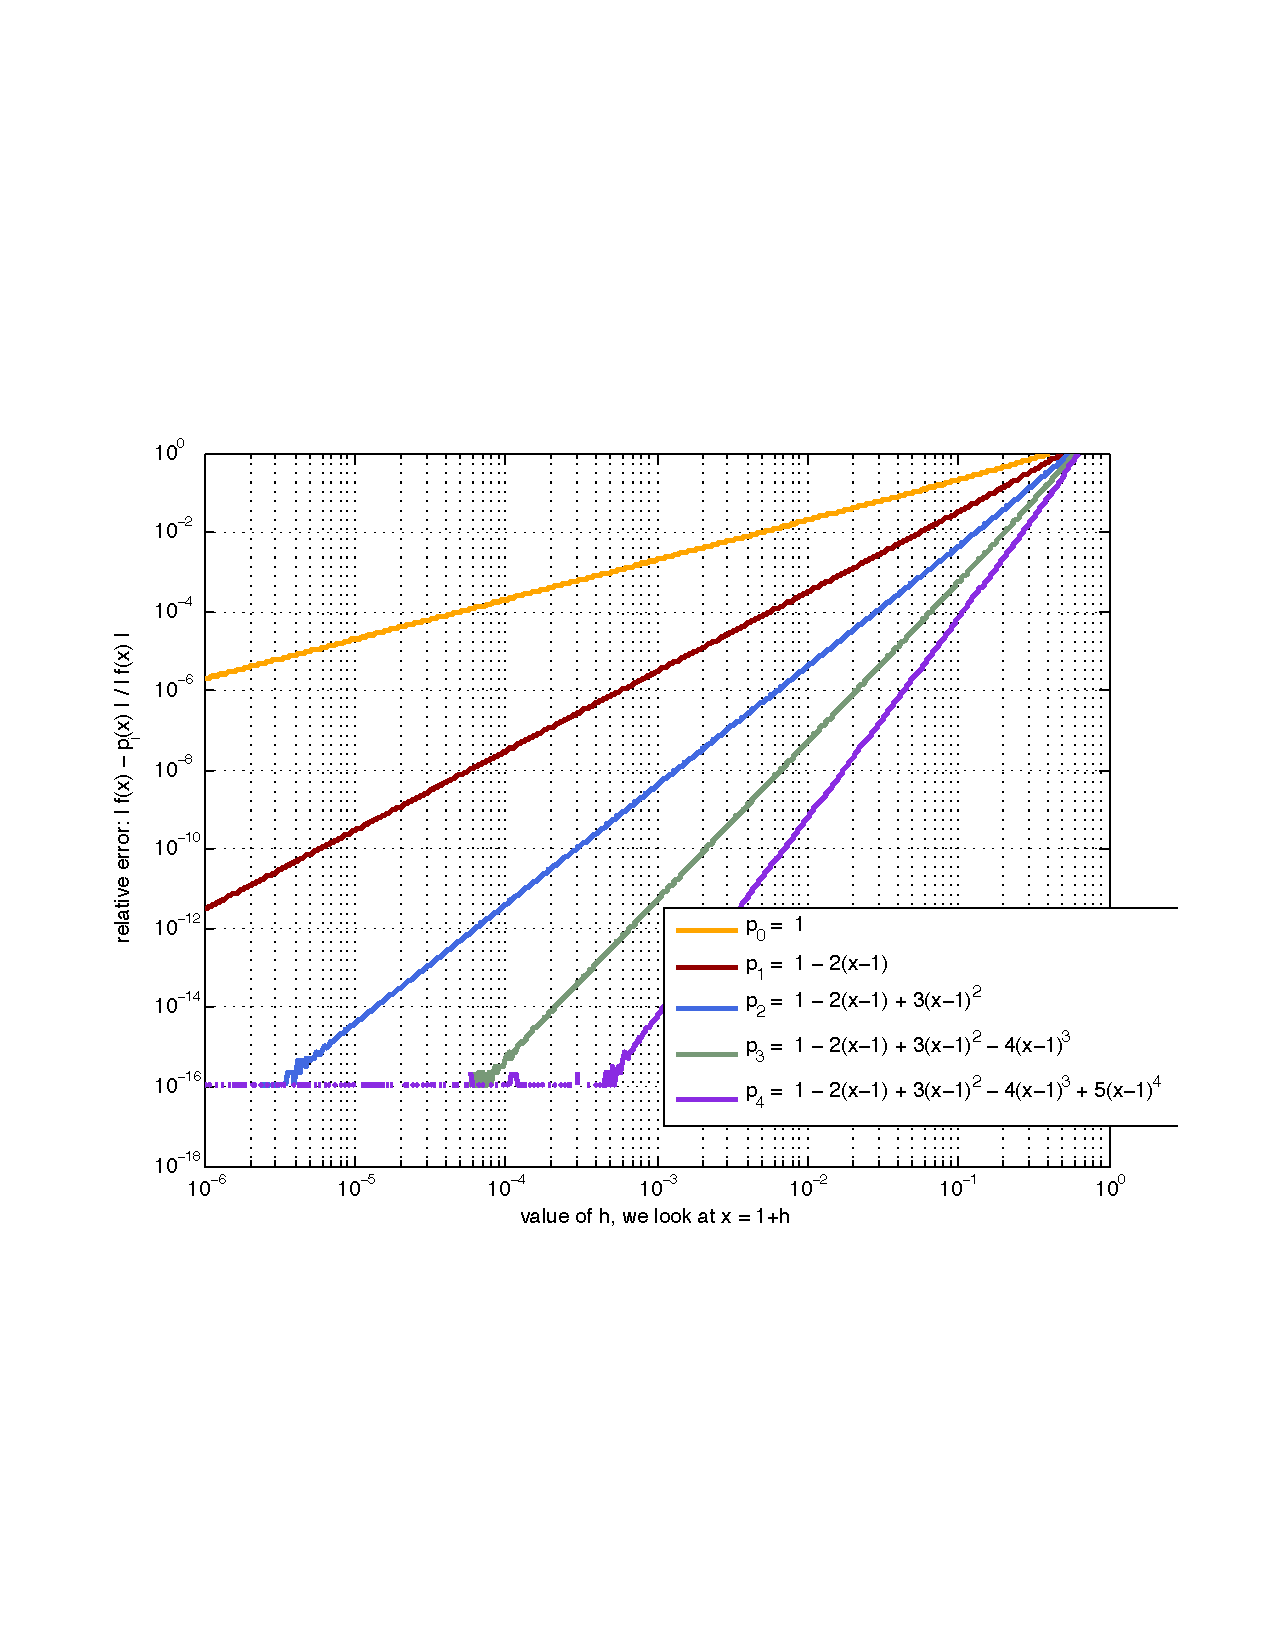
\includegraphics[width=.7\textwidth]{EX_0_5_6_fig5}


\end{document}
